\section{Trajectory Compression}
\label{sec:traj}
\subsection{Methods in Trajectory Compression blah}
A trajectory is a sequence of geospatial points that represents a path, optionally including a timestamp. The goal of compression is to reduce the size of the trajectory by storing it in a compressed form, while still containing the same information. This is measured by the compression ratio, which is the ratio between the uncompressed and compressed size and an accuracy metric, which determines to which degree information is retained. Additionally, trajectory compression can be classified into three main categories: streamed/batched, lossless/lossy, and spatial-only/spatio-temporal.

The primary distinction between streamed and batched compression lies in the amount of data processed at a time. Batched compression is generally simpler because it allows access to the entire trajectory at once. In contrast, streamed compression can only handle one segment at a time due to memory limitations, which prevents loading the entire trajectory. This limitation complicates the process as the complete scope of the trajectory remains unknown. A common approach for managing streamed data is the use of a Sliding Window, which forms the basis of many algorithms \cite{Sun2016}.

Batched compression, on the other hand, requires more storage and concentrated processing power. It necessitates loading the entire trajectory onto disk and processing it in a single operation. Due to its additional resource requirements and knowledge of the entire trajectory, batched compression outperforms streamed compression in terms of compression ratio and accuracy. Nonetheless, streamed compression can be advantageous in certain situations. Its ability to compress data as it is received, eliminating the need for intermediate storage, can outweigh the superior compression achieved by batched methods in terms of practicality. In addition, it is absolutely necessary for real time systems.

Lossy algorithms sacrifice accuracy for more efficient storage. Lossless algorithms reduce the size without losing any information. They generally have worse performance than lossy algorithms as a result of this. There is also category called \textit{Bounded Lossy Compression}, which was suggested by \textcite{zhao2018rest}. This allows compression algorithms to be lossy, but contained by an upper bound of "loss". The definition is stated by \textcite{zhao2018rest} as:

\begin{quote}
    \begin{definition}\label{def:bounded_lossy}
        Bounded Lossy Compression. Given a deviation $\epsilon$, an $\epsilon$-Bounded Lossy Compression algorithm transforms a raw trajectory $T$ into a compressed trajectory $T$, such that the distance between the reconstructed trajectory $T^*$ and $T$ does not exceed $\epsilon$, i.e., $d(T,T^*) \leq \epsilon$, where $d$ is some predefined distance function for trajectories.
    \end{definition}
\end{quote}

The distinction between spatial-only and spatio-temporal lies in the consideration of the temporal aspect, that is, whether time is taken into account or not. Spatial-only compression focuses solely on the spatial differences between trajectories. \textcite{SpatiotemporalComp}, define two spatio-temporal concepts that can improve trajectory compression: \textit{time-ratio distance} and \textit{speed difference threshold}.

The time-ratio distance represents the distance between two synchronized points: one point from the original trajectory and another point from the compressed trajectory. The traditional accuracy metric used in compression is the perpendicular distance between a point and the new trajectory. However, when using synchronized points the distance will change based on time. This was first defined by \textcite{SpatiotemporalComp} and has now been formalized under the term Synchronized Euclidean Distance (SED). Figure \ref{fig:sed} illustrates the concept of time-ratio distance, which will be further discussed in section \ref{subsub:SED}

The speed difference threshold is the concept of comparing speeds between sequential segments of the trajectory. The speed is not expected to be directly in the data; rather it is calculated as $ \Delta d / \Delta t $, where \textit{d} is distance and \textit{t} is time. When the speed difference is large this indicates a sudden movement or turn. These points are considered important for the internal shape of the trajectory. Therefore, ensuring no points with a speed difference larger than a certain threshold are removed during compression can increase the accuracy of the trajectory when considering the temporal aspect.

The results in the experiments by \textcite{SpatiotemporalComp} show that implementing time-ratio distance and a speed difference threshold had a slight improvement in compression ratio and a significant reduction of error. Although the accuracy metric was spatio-temporal and the algorithms used in comparison were not, therefore the results are not that surprising. Meanwhile, \textcite{Sun2016} claims that spatio-temporal is simple and efficient with the ability to maintain internal features in trajectories. However, they are unpopular because existing algorithms only consider speed which may lead to greater errors and break the holistic geometrical characteristics of trajectories.


\subsection{Accuracy Metrics}
The accuracy of a compression can be measured by different metrics. This is done by calculating some distance between each point in the original trajectory and the new trajectory. From these distances, various operations can be performed to obtain an overall metric. The mean distance of all points is the most commonly used measure, but other metrics such as median or maximum can also provide valuable insights into accuracy. The method used to calculate the distance, determines the accuracy metric. Example distances are shown in figure \ref{fig:sed}. The following sections will explore the most used accuracy metrics, as mentioned by, \textcite{TrajFramework} and \textcite{Sun2016}.

\subsubsection{Perpendicular Distance}
\label{subsec:PD}
Perpendicular distance (PD) refers to the shortest distance from a removed point to the new trajectory, as shown in figure \ref{fig:sed}. The shortest distance is always perpendicular to the trajectory, hence the name.

\subsubsection{Synchronized Euclidean Distance}
\label{subsub:SED}
SED is a measurement where a point $p_{i}$ is assigned a distance to the new trajectory that is equal to the distance to the synchronized point $p'_{i}$, as shown in figure \ref{fig:sed} $p'_{i}$ is calculated as:
\begin{equation}
    \begin{aligned}
        t'_{i} & = t_{i}                                                \\
        x'_{i} & = x_{s} + \frac{t_{i}-t_{s}}{t_{e}-t_{s}}(x_{e}-x_{s}) \\
        y'_{i} & = y_{s} + \frac{t_{i}-t_{s}}{t_{e}-t_{s}}(y_{e}-y_{s}) \\
    \end{aligned}
\end{equation}
This accuracy metric takes time into account. Two trajectories traversing the exact same spatial points might still be considered different if one took a longer time. This can be a useful metric for differentiating between taxi trips in rush hour and outside rush hour, since the trips outside rush hour will typically be shorter.

\begin{figure}[ht]
    \begin{minipage}[b]{0.49\linewidth}
        \centering
        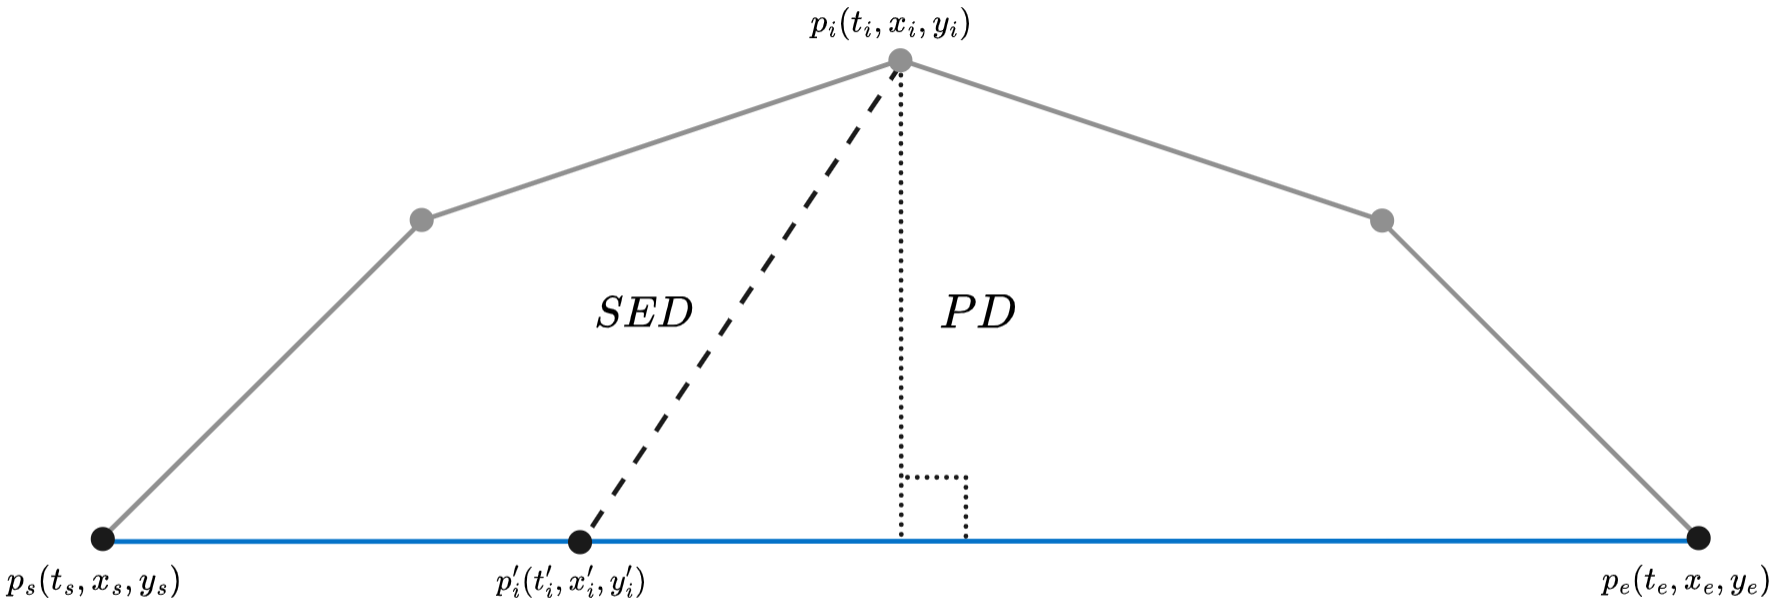
\includegraphics[width=\linewidth, height=7cm, keepaspectratio]{./figures/sed.png}
        \caption{Original trajectory in gray and new trajectory in blue showing distances SED and PD.}
        \label{fig:sed}
    \end{minipage}
    \begin{minipage}[b]{0.49\linewidth}
        \centering
        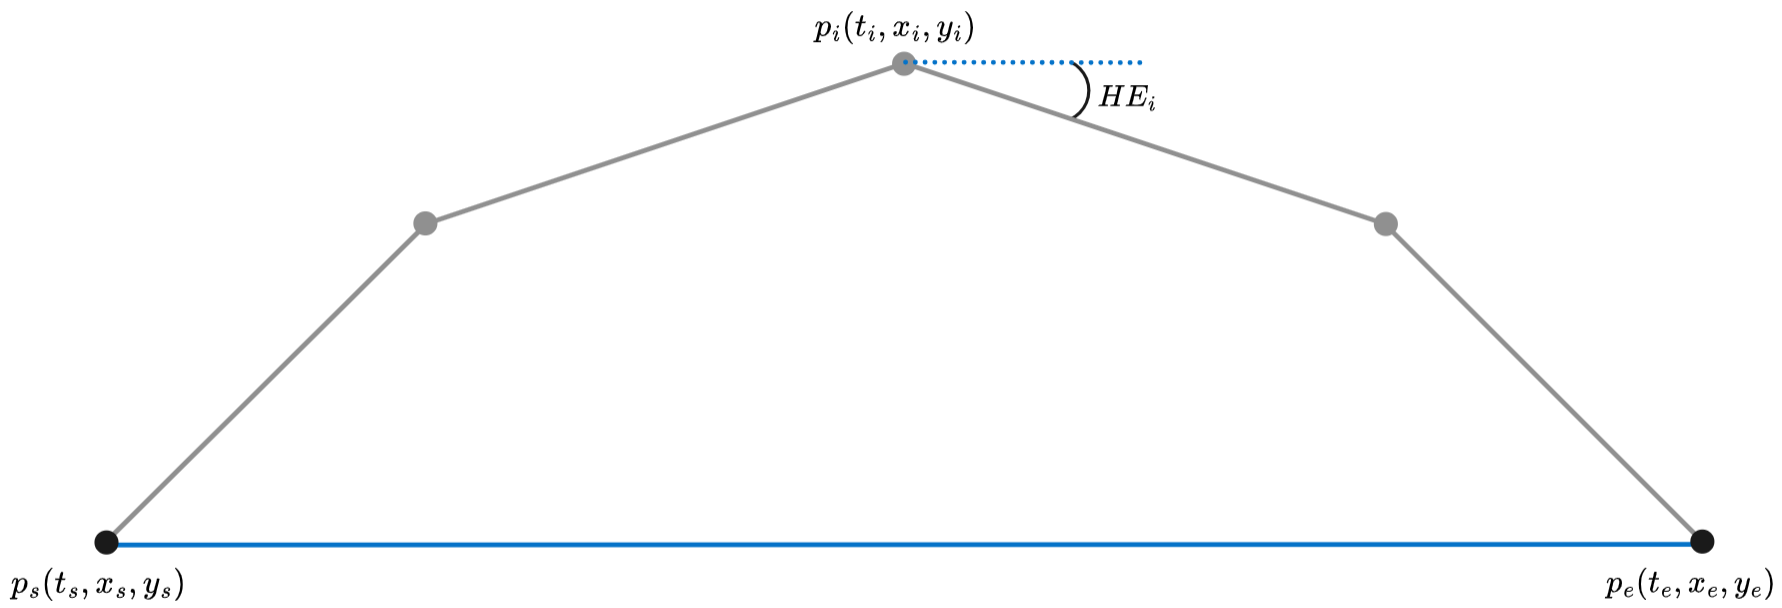
\includegraphics[width=\linewidth, height=7cm, keepaspectratio]{./figures/heading_error.png}
        \caption{Original trajectory in gray and new trajectory in blue showing distances HE.}
        \label{fig:hed}
    \end{minipage}
\end{figure}

\subsubsection{Heading Error}
The Heading Error (HE) for a point $p_{i}$ is the angular difference between the line segment $p_{i}$-$p_{i+1}$ along the original trajectory and $p'_{i}$-$p'_{i+1}$ along the compressed trajectory shown in figure \ref{fig:hed}. The angle represents the difference in direction between the original and the compressed trajectory at a given point. This metric is useful for detecting erratic movement and disruption of traffic flow according to \cite{TrajFramework}.

\subsubsection{Speed Error}
The Speed Error is similar to the Heading Error in that it compares the segments from the original trajectory with the corresponding segment in the compressed trajectory. However, it compares speed instead of direction. The Speed Error is the difference in speed between the original and compressed trajectory at a given point.

\subsection{Performance Metrics}
%Skrive no her? intro
\subsubsection{Compression Ratio}
Compression ratio measures the amount of data compressed. This is calculated as $C_{r} = \frac{|o|}{|c|}$, where $C_{r}$ is the compression ratio, $|o|$ is the size of the original data, and $|c|$ is the size of the compressed data. Storing a 10 GB file with 5 GB gives a compression ratio of $10 / 5 = 2$, meaning it was stored using half the original size. This can also be written as a 2:1 compression ratio.

\subsubsection{Compression Performance}
Compression performance measures the speed of compression as well as the resource usage. Compression speed is simply the time it took to compress measured. Resource usage, however can be measured in a variety of ways, this depends on what kind of usage you want to measure, for example memory usage or CPU time. Computer executions like these have variance in performance, therefore it is important to measure the average for multiple runs when doing an experiment, both for compression speed and resource usage. Additionally, it is important that when comparing compression performance that the measures were gathered in the same environment, meaning the experiment was executed on the same computer with the same version of the program. Otherwise, the results are not comparable.

\section{Dynamic Time Warping}
\label{sec:dtw}
According to \textcite{muller2007dynamic}, Dynamic Time Warping (DTW) is an algorithm used to determine the alignment cost between two temporal series. It can align the series by finding corresponding points between the series and finding the optimal alignment. The total alignment cost describes how similar the series are according to the DTW measure. When trying to align two different series, the alignment cost will be high, for two similar series, it will be low. Regarding trajectory compression, the alignment cost between a compressed trajectory and the original describes how similar they are, or how much information is preserved in the compressed form. A compression with high accuracy will have a low alignment cost.

There are many variations of DTW, that are made to speed up or otherwise improve it. We will begin by explaining Classical DTW from \textcite{muller2007dynamic}.

\subsection{Classical DTW}
Classical DTW works by calculating the cost matrix between two series. The cost $d_{i,j}$ in a matrix $D$ between the series $A$ and $B$ where \textit{distance} is a distance function between points, is given by:
\begin{equation}
    \label{eq:dtw}
    \begin{aligned}
        d_{i, j} & = distance(A_{i}, B_{j}) + \min \left\{ \begin{aligned}
                                                                & d_{i-1, j-1} \\
                                                                & d_{i-1, j}   \\
                                                                & d_{i, j-1}
                                                           \end{aligned} \right\}
    \end{aligned}
\end{equation}
\textcite{muller2007dynamic} introduces two terms, \textit{cost matrix} and \textit{accumulated cost matrix}. The cost matrix is a matrix of distances between all points in series $A$ and $B$, an example of a cost matrix is shown in figure \ref{fig:dtw_cost}. From the cost matrix, an accumulated cost matrix can be derived, each matrix cell contains the accumulated cost as defined in equation \ref{eq:dtw}. The accumulated cost matrix corresponding to the example in figure \ref{fig:dtw_cost} is shown in figure \ref{fig:dtw_acc_cost}. From equation \ref{eq:dtw} we see that the cost $d_{i, j}$ depends on the cost of previous points, for the first point $A_{1}$ and $B_{1}$ the previous points will not be defined. Therefore, a padding row and column is added: $d_{0,0} = 0$, $d_{1, 0}...d_{n, 0} = \infty$ and $d_{0, 1}...d_{0, m} = \infty$, this padding can be seen in figure \ref{fig:dtw_acc_cost}. The distance function depends on the type of data and the purpose of the DTW measure, Euclidean Distance or SED are common choices. The matrix cells are calculated one by one, from the top row, from left to right, using the cost function as described in equation \ref{eq:dtw}. Figure \ref{fig:dtw_acc_cost} shows an example of a DTW cost matrix for vectors $A = [8, 3, 7, 4, 3]$ and $B = [9, 5, 2, 6, 4]$. The total alignment cost is the accumulated cost in the final cell, $d_{5,5}$ in figure \ref{fig:dtw_acc_cost}, or more generally $d_{n,m}$.

Additionally, \textcite{muller2007dynamic} introduces the term \textit{warping path}, which is a sequence of points (matrix cells) in an accumulated cost matrix, that defines alignment between two sequences. If a warping path for $A$ and $B$ in the matrix $M$, includes $M_{1,2}$ this represents aligning point $A_1$ to $B_2$. The \textit{optimal warping path} is the warping path with the lowest total cost among all possible warping paths \cite{muller2007dynamic}. To find the optimal warping path, start from the last cell of the matrix and trace back to the first, selecting the paths with the lowest costs. If there are ties in cost, a predetermined set of priorities for different path directions (diagonal, horizontal, vertical) is used. Consequently, there can be multiple warping paths with the same minimal cost, but only one optimal warping path. Figure \ref{fig:dtw_acc_cost} shows the optimal warping path drawn in the accumulated cost matrix.

\begin{figure}[h]
    \centering
    \begin{tabular}{|c|c|c|c|c|c|c|}
        \hline
        \multicolumn{1}{|c|}{\diagbox{$A_{i}$}{$B_{j}$}} &          & 9        & 5        & 2        & 6        & 4        \\ \hline
                                                         & 0        & $\infty$ & $\infty$ & $\infty$ & $\infty$ & $\infty$ \\ \hline
        8                                                & $\infty$ & 1        & 3        & 6        & 2        & 4        \\ \hline
        3                                                & $\infty$ & 6        & 2        & 1        & 3        & 1        \\ \hline
        7                                                & $\infty$ & 2        & 2        & 5        & 1        & 3        \\ \hline
        4                                                & $\infty$ & 5        & 1        & 2        & 2        & 0        \\ \hline
        3                                                & $\infty$ & 6        & 2        & 1        & 3        & 1        \\ \hline
    \end{tabular}
    \caption{The DTW cost Matrix $M$ between vectors $A = [8, 3, 7, 4, 3]$ and $B = [9, 5, 2, 6, 4]$. The distance function for these one dimensional points is simply the absolute value of the difference. The blue line shows the optimal path between the vectors.
    }
    \label{fig:dtw_cost}
\end{figure}
\begin{figure}
    \centering
    \begin{tabular}{|c|c|c|c|c|c|c|}
        \hline
        \multicolumn{1}{|c|}{\diagbox{$A_{i}$}{$B_{j}$}} &                    & 9        & 5                & 2                  & 6        & 4                  \\ \hline
                                                         & 0\tikzmark{start1} & $\infty$ & $\infty$         & $\infty$           & $\infty$ & $\infty$           \\ \hline
        8                                                & $\infty$           & 1        & 3                & $6$                & $2$      & $4$                \\ \hline
        3                                                & $\infty$           & 7        & 3\tikzmark{end1} & $4$\tikzmark{end2} & $5$      & $3$                \\ \hline
        7                                                & $\infty$           & 9        & 5                & $8$                & $5$      & $6$                \\ \hline
        4                                                & $\infty$           & 14       & 6                & $7$                & $7$      & $5$\tikzmark{end3} \\ \hline
        3                                                & $\infty$           & 20       & 8                & $7$                & $10$     & $6$\tikzmark{end4} \\ \hline
    \end{tabular}
    \caption{The DTW accumulated cost Matrix $M$ for vectors $A = [8, 3, 7, 4, 3]$ and $B = [9, 5, 2, 6, 4]$. The costs are based on the cost matrix in figure \ref{fig:dtw_cost}. The blue line shows the optimal path between the vectors. The optimal alignment from $A$ to $B$ is $[8\rightarrow9, 3\rightarrow(5, 2), 7\rightarrow6, 4\rightarrow4, 3\rightarrow4]$. The alignment cost (or DTW distance) is the value in the last matrix cell, in this case $M_{5,5} = 6$.}
    \label{fig:dtw_acc_cost}
    \begin{tikzpicture}[overlay, remember picture]
        \draw[thick, blue, -, opacity=0.7] ($(pic cs:start1) + (0.05,-6.3)$) -- ($(pic cs:end1) + (0.05,-6.3)$);
        \draw[thick, blue, -, opacity=0.7] ($(pic cs:end1) + (0.05,-6.3)$) -- ($(pic cs:end2) + (0.05,-6.3)$);
        \draw[thick, blue, -, opacity=0.7] ($(pic cs:end2) + (0.05,-6.3)$) -- ($(pic cs:end3) + (-0.2,-6.3)$);
        \draw[thick, blue, -, opacity=0.7] ($(pic cs:end3) + (-0.2,-6.3)$) -- ($(pic cs:end4) + (-0.2,-6.3)$);
    \end{tikzpicture}
\end{figure}

\textcite{muller2007dynamic} discusses several ways to improve classical DTW, such as modifying the cost function to reduce the number of vertical and horizontal lines in the optimal path, thereby preventing the path from getting stuck on one sequence. One approach involves implementing lower weights for diagonal movements or altering the cost function to incorporate more of the previous points.

Additionally, \textcite{muller2007dynamic} describes techniques to speed up classical DTW by coarsening data or by using global constrains. Coarsening the data allows for an initial rough estimation of the optimal path, followed by a more precise calculation in the selected areas of the matrix. Global constraints, such as the Sakoe-Chiba band and the Itakura parallelogram eliminate parts of the matrix \cite{muller2007dynamic}. This requires less computation and ensures that the optimal path stays within some proximity to the main diagonal. The Sakoe-Chiba is discussed later in section 3.1.

One challenge with DTW is that distances varies with the length of the vectors. The distance between longer vectors tend to be greater than for shorter vectors. This happens because the total alignment cost adds up the costs for all previous points along the optimal path. Consequently, more points lead to a higher alignment cost even if the trajectories are very similar. To address this issue, normalized versions of DTW have been proposed, such as Average DTW and Max DTW \cite{zhao2018rest}. MaxDTW in particular will be explained in the following section.

\subsection{Max DTW}
\textcite{zhao2018rest} introduced Max Dynamic Time Warping (MaxDTW), a variant of classical DTW that accounts for the lengths of the vectors (trajectories). MaxDTW changes the cost function by taking the max of the distance and the former points minimum instead of taking the sum like in equation \ref{eq:dtw}. The new cost function is
\begin{equation}
    \label{eq:max_dtw}
    \begin{aligned}
        d_{i, j} & = max(distance(A_{i}, B_{j}), \min \left\{ \begin{aligned}
                                                                   & d_{i-1, j-1} \\
                                                                   & d_{i-1, j}   \\
                                                                   & d_{i, j-1}
                                                              \end{aligned} \right\})
    \end{aligned}
\end{equation}
This new cost function does not accumulate like in classical DTW, it simply represents the worst alignment of the optimal path to the current cell. The final cost represents the highest cost for a single alignment along the optimal path for the vectors. An example of a MaxDTW cost matrix is shown in figure \ref{fig:max_dtw}, the vectors $A$ and $B$ are the same as in figure \ref{fig:dtw_acc_cost}. Here we can see that the end $M_{5,5} = 2$, this represents the highest cost along the optimal path, which is aligning $A_2 = 3$ to $B_2 = 5$, the cost $|A_2 - B_2| = 2$ is also the total cost for the vectors when applying MaxDTW.
\begin{figure}[t!]
    \centering
    \begin{tabular}{|c|c|c|c|c|c|c|}
        \hline
        \multicolumn{1}{|c|}{\diagbox{$A_{i}$}{$B_{j}$}} &                    & 9        & 5                & 2                  & 6        & 4                  \\ \hline
                                                         & 0\tikzmark{start1} & $\infty$ & $\infty$         & $\infty$           & $\infty$ & $\infty$           \\ \hline
        8                                                & $\infty$           & 1        & 3                & $6$                & $6$      & $6$                \\ \hline
        3                                                & $\infty$           & 6        & 2\tikzmark{end1} & $2$\tikzmark{end2} & $3$      & $3$                \\ \hline
        7                                                & $\infty$           & 6        & 2                & $5$                & $2$      & $3$                \\ \hline
        4                                                & $\infty$           & 6        & 2                & $2$                & $2$      & $2$\tikzmark{end3} \\ \hline
        3                                                & $\infty$           & 6        & 2                & $2$                & $3$      & $2$\tikzmark{end4} \\ \hline
    \end{tabular}
    \begin{tikzpicture}[overlay, remember picture]
        \draw[thick, blue, -, opacity=0.7] ($(pic cs:start1) + (-0.0,0.15)$) -- ($(pic cs:end1) + (-0.1,0.1)$);
        \draw[thick, blue, -, opacity=0.7] ($(pic cs:end1) + (-0.1,0.1)$) -- ($(pic cs:end2) + (-0.1,0.1)$);
        \draw[thick, blue, -, opacity=0.9] ($(pic cs:end2) + (-0.1,0.1)$) -- ($(pic cs:end3) + (-0.25,0.05)$);
        \draw[thick, blue, -, opacity=1] ($(pic cs:end3) + (-0.25,0.05)$) -- ($(pic cs:end4) + (-0.25,0.05)$);
    \end{tikzpicture}
    \caption{The MaxDTW accumulated cost matrix $M$ for vectors $A = [8, 3, 7, 4, 3]$ and $B = [9, 5, 2, 6, 4]$. The costs are based on the cost matrix in figure \ref{fig:dtw_cost}. The blue line shows the optimal path between the vectors. The optimal alignment from $A$ to $B$ is $[8\rightarrow9, 3\rightarrow(5, 2), 7\rightarrow6, 4\rightarrow4, 3\rightarrow4]$. The alignment cost (or MaxDTW distance) is the value in the last matrix cell, in this case $M_{5,5} = 2$.
    }
    \label{fig:max_dtw}
\end{figure}

MaxDTW is sensitive to outliers points because a single poor alignment can significantly increase the total alignment cost. Additionally, this measure does not indicate whether there are many points close to the alignment max or just one. This makes MaxDTW most useful to test threshold conditions. For instance, an application where no point can have an alignment cost above a certain threshold. MaxDTW is also normalized and can be used to compare distances for sequences of varying lengths.

\subsection{Sakoe-Chiba Band}
\label{sec:sakoe}
The Sakoe-Chiba Band was suggested by \textcite{sakoe1978dynamic} as a global constraint that restricts the matrix comparison area. This is not a specific DTW variant in itself, but is a simplification that can be applied to any DTW calculation. The accessible region of the matrix is a band drawn around the main diagonal. This can be seen in figure \ref{fig:dtw_band}, where the inaccessible area is gray.

This band reduces the runtime of the calculation, but also reduces the precision of the result. The band is centered around the diagonal and will therefore be most successful for series where the optimal warping path stays close to the diagonal \cite{sakoe1978dynamic}. This applies to series that are quite similar in length and location. Note that for series of dissimilar length the total cost will not necessarily be in $M_{n,m}$, but in the cell within the band size around the main diagonal that is closest to $M_{n,m}$. Distances in the matrix are calculated in Manhattan distance. As shown in Figure \ref{fig:dtw_band}, cells that are diagonal to the main diagonal do not fall within the band because their Manhattan distance from the main diagonal is two, while the band size is one.

\begin{figure}
    \centering
    \begin{tabular}{|c|c|c|c|c|c|c|}
        \hline
        \multicolumn{1}{|c|}{\diagbox{$A_{i}$}{$B_{j}$}} &                           & 9                   & 5                        & 2                         & 6                         & 4                         \\ \hline
                                                         & 0\tikzmark{start1}        & $\infty$            & $\infty$\cellcolor{gray} & $\infty$ \cellcolor{gray} & $\infty$ \cellcolor{gray} & $\infty$ \cellcolor{gray} \\ \hline
        8                                                & $\infty$                  & 1                   & 3                        & 6 \cellcolor{gray}        & 2 \cellcolor{gray}        & 4 \cellcolor{gray}        \\ \hline
        3                                                & $\infty$ \cellcolor{gray} & 7                   & 3\tikzmark{end1}         & $4$\tikzmark{end2}        & 5 \cellcolor{gray}        & 3 \cellcolor{gray}        \\ \hline
        7                                                & $\infty$ \cellcolor{gray} & 9 \cellcolor{gray}  & 5                        & $8$                       & $5$                       & 6 \cellcolor{gray}        \\ \hline
        4                                                & $\infty$ \cellcolor{gray} & 14 \cellcolor{gray} & 6 \cellcolor{gray}       & $7$                       & $7$                       & $5$\tikzmark{end3}        \\ \hline
        3                                                & $\infty$ \cellcolor{gray} & 20 \cellcolor{gray} & 8  \cellcolor{gray}      & 7 \cellcolor{gray}        & $10$                      & $6$\tikzmark{end4}        \\ \hline
    \end{tabular}
    \caption{The DTW accumulated cost Matrix $M$ for vectors $A = [8, 3, 7, 4, 3]$ and $B = [9, 5, 2, 6, 4]$ with a Sakoe-Chiba band of size 1 applied. The grey area is inaccessible for comparison. This can also be seen as setting the costs in the gray area to $\infty$.}
    \label{fig:dtw_band}
    \begin{tikzpicture}[overlay, remember picture]
        \draw[thick, blue, -, opacity=0.7] ($(pic cs:start1) + (-0.1,0.1)$) -- ($(pic cs:end1) + (-0.1,0.1)$);
        \draw[thick, blue, -, opacity=0.7] ($(pic cs:end1) + (-0.1,0.1)$) -- ($(pic cs:end2) + (-0.1,0.1)$);
        \draw[thick, blue, -, opacity=0.7] ($(pic cs:end2) + (-0.1,0.1)$) -- ($(pic cs:end3) + (-0.1,0.1)$);
        \draw[thick, blue, -, opacity=0.7] ($(pic cs:end3) + (-0.1,0.1)$) -- ($(pic cs:end4) + (-0.1,0.1)$);
    \end{tikzpicture}
\end{figure}